\question \textbf{Questions from Quiz 8}

\begin{parts}

    \part Electric car sales in 2018 were $\sim$1.5 million/yr and have recently been doubling every 1.5 yr.
        $2^{10} \approx 1000$. Most likely, by when will everyone buy an electric car each year on average?

    \begin{choices}
        \choice 2050-2070
        \choice 2030-2035
        \choice 2040-2050
        \choice 2035-2040
        \correctchoice Never, because it would be absurd for every person to buy a car every year.
    \end{choices}

    \begin{solution}
        Slide ``Acceleration can't continue'', says: ``For those examples, there are limits. Doubling can't go on.
        May slow to linear increase, no increase (S-curve), decrease.'' Common sense should tell that we're
        not all going to buy a car every year because that would be far too expensive, would waste an
        enormous amount of resources, and would totally jam streets and parking. Imagine Hong Kong with
        8 million new cars each year! Thus, without even doing any math, it's obvious that the likely answer
        is ``never''. This seems like a trick question, and in a way it is. But a key point of both the chapter and
        the lecture is that trends often don't continue.
    \end{solution}

    \part The greatest number of people were/are/will be added to the middle class (US\$11-110/day) annually around

    \begin{oneparchoices}
        \choice 2040
        \choice 2000
        \correctchoice now
        \choice 1980
        \choice 1960
    \end{oneparchoices}

    \begin{solution}
        Slide ``Consumer explosion: Middle class growing'' says, ``Fastest growth
        in middle class is this generation.''. I also emphasized this by saying in the lecture something to the
        effect that the middle class will grow the most around these few decades.
    \end{solution}

    \part What is the Fermi Paradox?

    \begin{choices}
        \choice The chain reaction in nuclear bombs should continue until the world is destroyed, yet it stops before then.
        \choice There are many Great Filters, yet we developed a civilization.
        \choice This statement is false.
        \correctchoice If many places could develop life, why haven't we contacted aliens?
        \choice One can know something's position or velocity, but not both.
    \end{choices}

    \begin{solution}
        If many places could develop life, why haven't we contacted aliens? This was from the video on the
        last slide.
    \end{solution}

    \part Ridley feels that the most important factor in the long-term acceleration of economic development has been

    \begin{choices}
        \choice more research into basic phenomena of nature.
        \choice accelerating efforts by countries to foster innovation in key industries.
        \choice rising legal protection of new knowledge.
        \correctchoice higher rate of mixing of various concepts.
        \choice the increasing amount of money invested.
    \end{choices}

    \begin{solution}
        Ridley asks if innovation driving the world is from expansion of science, application of money,
        granting of intellectual property or something more bottom-up. He rejects all as major factors
        except the last: exchange, or mixing.
    \end{solution}

    \part What is likely the most important reason for the rapid advance of civilization in the last few centuries?

    \begin{choices}
        \choice The communication implosion
        \choice Malthusian Trap
        \choice Fermi Paradox
        \correctchoice The demographic transition
        \choice Moore's Law
    \end{choices}

    \begin{solution}
        The common cause for the producer and consumer explosion is the demographic transition. The
        producer and consumer explosion (together with the communication explosion and increase in the
        development of tools) were the biggest factors in the accelerated innovation post-1800s.
    \end{solution}

    \part What does Ridley feel is most remarkable about the last 2 centuries?

    \begin{oneparchoices}
        \choice nuclear bombs
        \correctchoice compounding success
        \choice advances in science
        \choice Moore's law
        \choice vastly better health
    \end{oneparchoices}

    \begin{solution}
        In The Rational Optimist, Ridley says: ``The most fundamental feature of the modern world since
        1800 - more profound than flight, radio, nuclear weapons or websites, more momentous than
        science, health, or material well-being - has been the continuing discovery of `increasing returns'.''
    \end{solution}

    \part The increased ability of people to buy goods and services over the last couple of centuries is

    \begin{oneparchoices}
        \correctchoice the Consumer explosion.
        \choice the Singularity.
        \choice Moore's law.
        \choice the Producer explosion.
        \choice Wright's law.
    \end{oneparchoices}

    \begin{solution}
        Consumer explosion (see slide ``Consumer explosion: many more people'')
    \end{solution}

    \part Which is most accurate about intellectual property?

    \begin{choices}
        \correctchoice When patent thickets exist, they draw away profits of new inventions to the last patent
        holder to relent during negotiation.
        \choice Without patents, inventors are not motivated to invent.
        \choice Intellectual property is most beneficial to the inventor if she protects it and keeps it to
        herself.
        \choice Intellectual properties can explain why some places are more innovative than others.
        \choice Patent trolls are firms that obstruct the patent system by failing to sue others infringing on
        their patents.
    \end{choices}

    \begin{solution}
        A patent thicket occurs when each step in a metabolic
        pathway is subject to a patent, When encountering a patent thicket, according to The
        Rational Optimist, ``a medical inventor can find himself negotiating away all his rewards
        before he even tests his idea. And the last patent holder to yield commands the highest
        potential pay-off.''
    \end{solution}

    \part Which one of the following statements concerning government funding for research is FALSE:

    \begin{choices}
        \choice The US government created Sematech to improve American competitiveness in the
        memory chip market.
        \correctchoice Since the mid-20th century, annual US government spending on research and
        development has been consistently greater than that of the private sector.
        \choice Government funded GPS.
        \choice Government funding resulted in the creation of the internet.
        \choice Government funding led to human exploration of the moon.
    \end{choices}

    \begin{solution}
        It is false that, since the mid-20th century, total US government spending on R\&D has been
        greater than that of the private sector. Slide ``Government? US R\&D funding'' clearly shows
        that private sector R\&D funding as a \% of GDP has been greater since the 1980s.
    \end{solution}

    \part How has the producer explosion accelerated innovation?

    \begin{choices}
        \choice It sped the flow of information.
        \choice It started a second demographic transition.
        \choice It broke through the Great Filter.
        \correctchoice It increased the time and resources for invention.
        \choice It created demand for a greater variety of inventions, and a greater number of each invention.
    \end{choices}

    \begin{solution}
        Slide ``Producer explosion''
    \end{solution}

    \part According to Matt Ridley, what was the major factor that made economists' predictions
        about the eventual stagnation of the economy wrong?

    \begin{choices}
        \choice Experts predicted that fossil fuels would soon be depleted, stopping economic growth.
        However, more and more fossil fuels have been discovered.
        \choice Economists predicted that the future economy will be conquered by monopolies, but the
        idea of open competitive markets eventually spread over the world and thus made their
        predictions wrong.
        \correctchoice Economists assumed that an equilibrium state exists, but innovations make the steady-
        state impossible and thus made their predictions wrong.
        \choice Economists thought that trade would be heavily concentrated locally, but nowadays trade
        often crosses the world.
        \choice Economists like Adam Smith foresaw that every government will eventually seize control
        of every market, but it turned out that a free economy had become the mainstream.
    \end{choices}

    \begin{solution}
        The answer is that economists assumed that an equilibrium state exists, but the possibility of
        new knowledge and innovations make the steady-state impossible and thus made their
        predictions wrong. The introduction to Chapter 8 of The Rational Optimist: ``Nobody
        predicted this. The pioneers of political economy expected eventual stagnation. Adam Smith,
        David Ricardo and Robert Malthus all foresaw that diminishing returns would eventually set
        in, that the improvement in living standards they were seeing would peter out...The
        possibility of new knowledge makes the steady state impossible. Somewhere somebody will
        have a new idea and that idea will enable him to invent a new combination of atoms both to
        create and to exploit imperfections in the market.''
        
        The other choices are logically correct and related to the course, but they do not cover
        Ridley's main point of view in Chapter Eight of The Rational Optimist.
    \end{solution}

    \part For your group presentation, you want to show the global distribution of your country's oil
        export destinations, emphasizing comparisons of amounts among the 8 countries you export
        to. Which graph/chart should you use?

    \begin{choices}
        \choice Pie chart
        \correctchoice Bar graph
        \choice None. A table would be better so that you can state the exact amounts.
        \choice Line graph
        \choice Scatter plot
    \end{choices}

    \begin{solution}
        A bar graph would work best because you can readily compare amounts. It would be
        harder to compare amounts on a pie chart because each slice starts in a different position; also trying
        to distinguish 8 colors to read the pie chart would waste time. A table just shows text, which is harder
        to comprehend at a glance, and showing so many digits would be uninformative and distracting.
        Scatter or line plots are better for comparing 2 quantitative dimensions, not 1 quantitative and 1
        categorical dimension.
    \end{solution}

    \part Early copper axes were as thick as stone axes, and only later were made thinner, which
        Ridley mentions to illustrate that

    \begin{choices}
        \choice violence was more common then, requiring more sturdy weapons.
        \choice they were decorative.
        \choice as technology progresses, design still follows the human form.
        \correctchoice ideas often come from other ideas.
        \choice agriculture supported a richer, denser population than did hunting and gathering.
    \end{choices}

    \begin{solution}
        In Chapter 8 of The Rational Optimist, Ridley said that ``objects betray in their design
        their descent from other objects: ideas that have given birth to other ideas. The first copper axes of
        5,000 years ago were the same shape as the polished stone tools then in common use. Only later did
        they become much thinner as the properties of metals became better understood.''
        
        The answer, ``after a revolution in innovation, evolution then improves on it'', makes sense, but is not why Ridley
        mentioned this observation about early copper axes.
    \end{solution}

    \part Which of the following graphs is most effective in supporting the following information:
        ``Thailand is an oil-producing country, yet it increasingly relies on crude oil imports due to high demand''?

    \begin{figure}[H]
        \centering
        \begin{subfigure}{0.25\linewidth}
            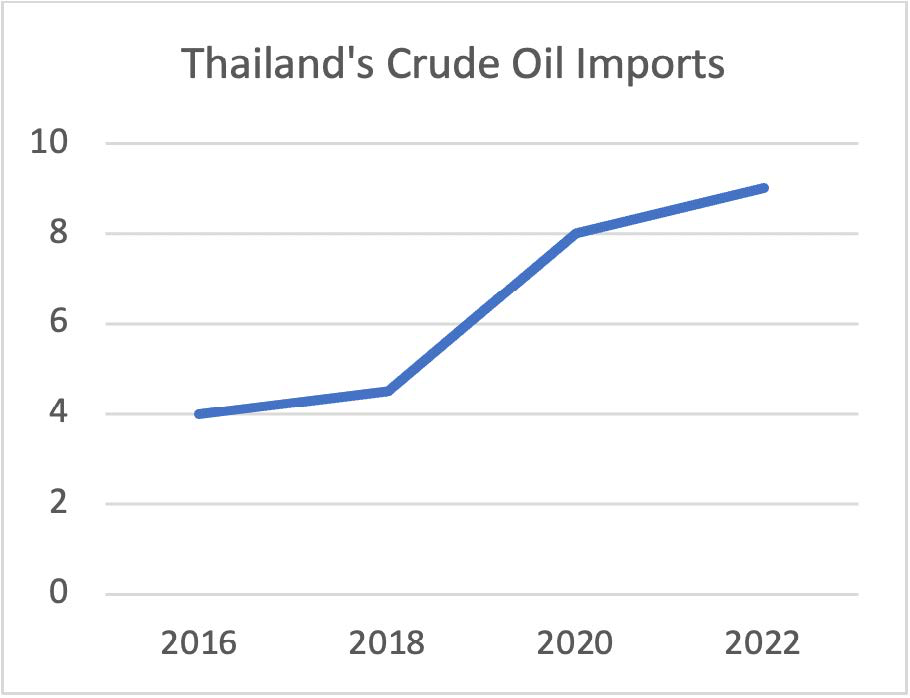
\includegraphics[width=\textwidth]{figs/quiz8-thailand-optA.png}
            \caption{ }
        \end{subfigure}
        \hspace{0.5cm}
        \begin{subfigure}{0.25\linewidth}
            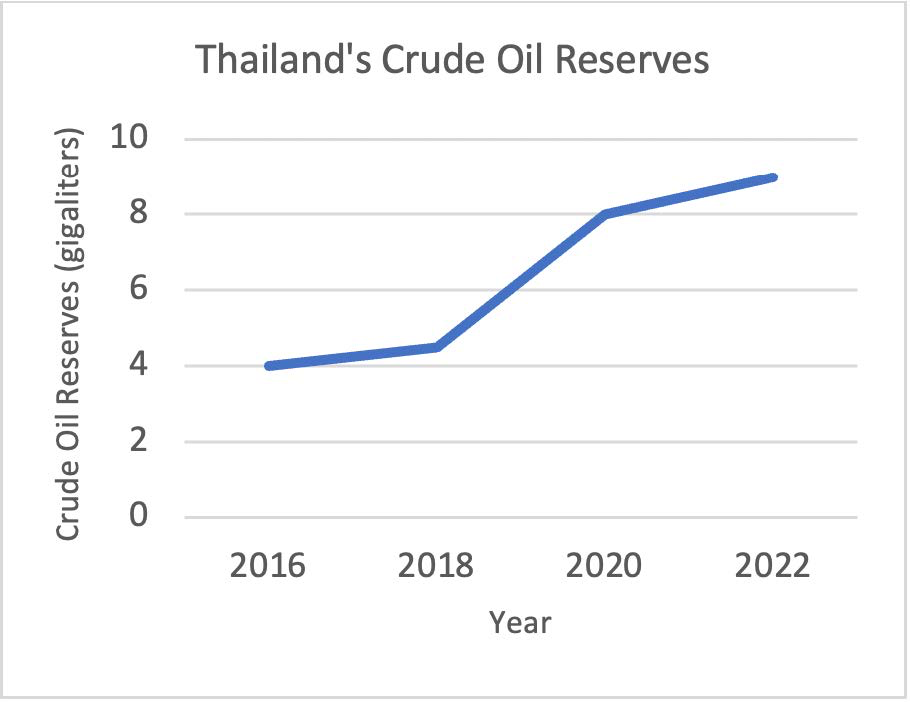
\includegraphics[width=\textwidth]{figs/quiz8-thailand-optB.png}
            \caption{ }
        \end{subfigure}
        \hspace{0.5cm}
        \begin{subfigure}{0.25\linewidth}
            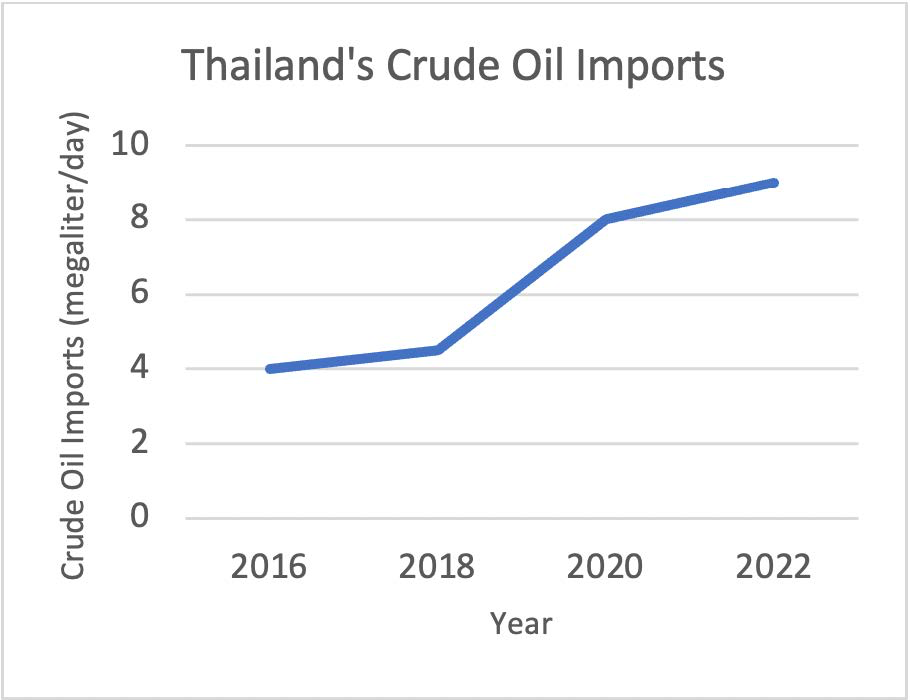
\includegraphics[width=\textwidth]{figs/quiz8-thailand-optC.png}
            \caption{ }
        \end{subfigure}
        \hspace{0.5cm}
        \begin{subfigure}{0.25\linewidth}
            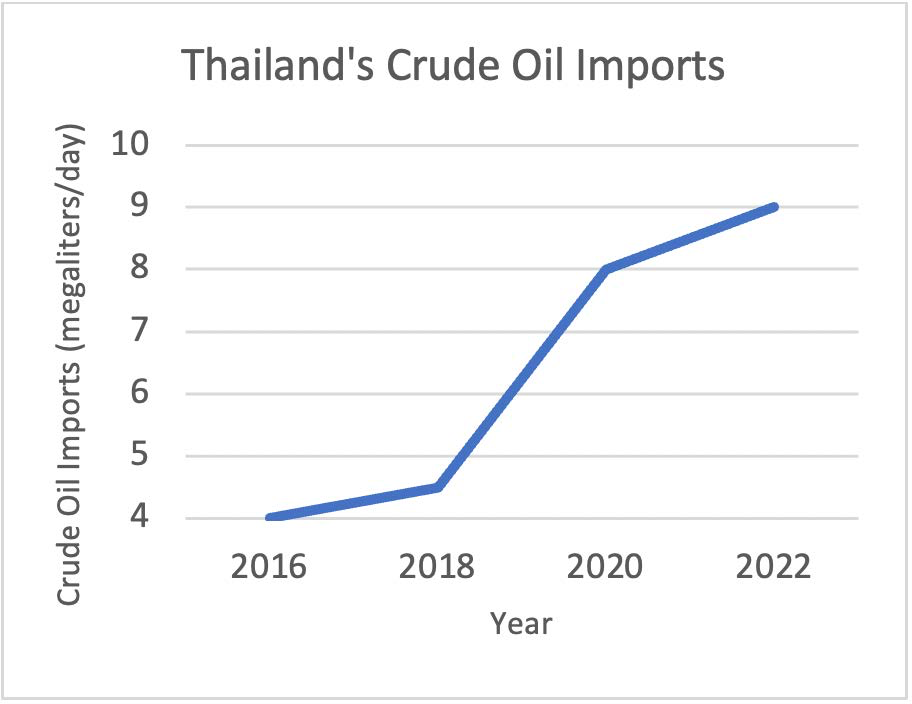
\includegraphics[width=\textwidth]{figs/quiz8-thailand-optD.png}
            \caption{ }
        \end{subfigure}
        \hspace{0.5cm}
        \begin{subfigure}{0.25\linewidth}
            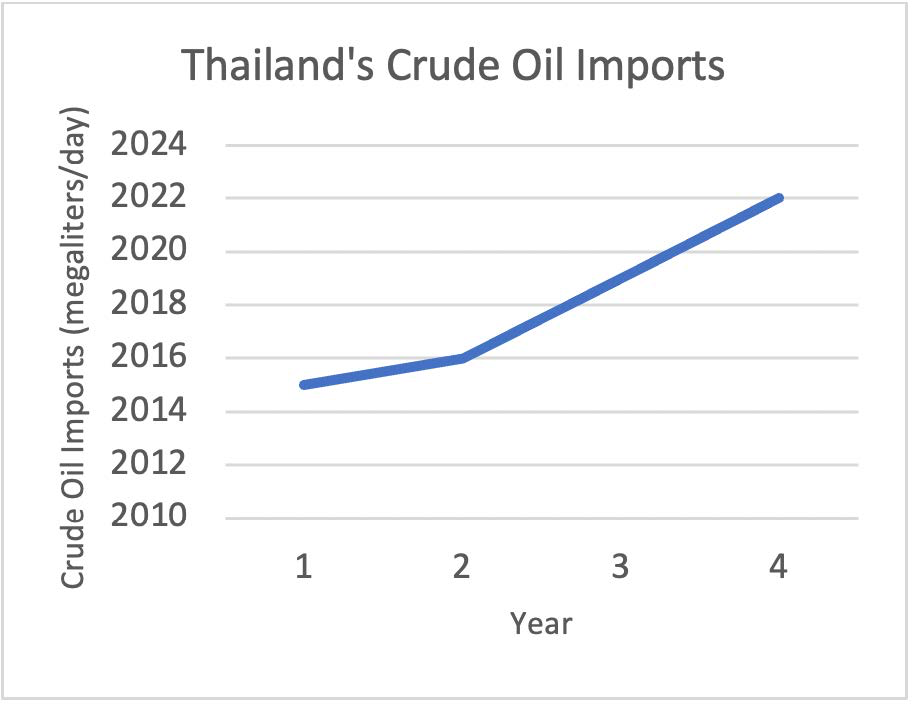
\includegraphics[width=\textwidth]{figs/quiz8-thailand-optE.png}
            \caption{ }
        \end{subfigure}
    \end{figure}
    
    \begin{oneparchoices}
        \choice (1)
        \choice (2)
        \correctchoice (3)
        \choice (4)
        \choice (5)
    \end{oneparchoices}

    \begin{solution}
        When displaying information on a graph, pay attention to the presence of units,
        consistency of time interval, usually starting the vertical axis at zero, and the accuracy of the graph
        little.
    \end{solution}

    \part Which statement is most accurate?

    \begin{choices}
        \choice In the video, ``Connections'', Burke said that his favorite influence for change is deliberate search.
        \choice Moore's Law is a lot more accurate than Wright's Law.
        \choice The hype cycle is a feedback loop in which AI hyper-accelerates innovation.
        \choice The internet was the biggest factor accelerating innovation during the 1800s.
        \correctchoice Wright's Law is a little more accurate than Moore's Law.
    \end{choices}

    \begin{solution}
        The correct answer is that Wright's Law is a little more accurate than Moore's Law
        (slide ``Is Moore's Law unique to chips?'').
        
        Burke said (14:26 in ``Connections'' video) that his favorite
        influence for change is surprise use of one thing in another field, not deliberate search (which he said
        was a bore in the case of Edison's light bulb).
        
        Most innovations have come from the private sector.
        The hype cycle is not an AI feedback loop (``Hype cycle'' slide). 
        
        The biggest factors in innovation
        acceleration are the producer explosion and customer explosion, not communication (slides titled
        ``Why has change increased?'').
        
        The internet didn't exist in the 1800s.
    \end{solution}

    \part According to the lecture, why do we sometimes reject innovation?

    \begin{choices}
        \choice Innovation sometimes violates the Fermi Paradox.
        \choice Acceleration can't continue.
        \choice Innovation increases income inequality (the 4 ``I'').
        \correctchoice People may want to maintain their traditions.
        \choice Results of innovation can only be enjoyed by the upper class in society.
    \end{choices}

    \begin{solution}
        The answer is that we want to maintain traditions. See slide ``Anti-change'' and video ``Tradition!''.
    \end{solution}

    \part What is Matt Ridley trying to explain with ``Thomas Jefferson's candle''?

    \begin{choices}
        \choice The improvement of lighting by Jefferson's time illustrated that everyone could live like the rich of centuries past.
        \correctchoice Knowledge spreads easily.
        \choice Electricity produced new knowledge.
        \choice Discoveries about the physics of combustion have led to the industrial revolution.
        \choice Only rich people like Jefferson could afford candles.
    \end{choices}

    \begin{solution}
        ``Thomas Jefferson's candle'' can light other candles without darkening itself.
        This is a metaphor showing that old knowledge is shared and used to produce new knowledge without being destroyed.
    \end{solution}

    \part Which of these statements concerning Moore's law is most accurate?

    \begin{choices}
        \choice Moore's law is more accurate than Wright's law.
        \choice Moore's law was proposed by the founder of Microsoft.
        \choice Moore himself has outlived his law.
        \choice Moore's Law states that the price of electronic chips will increase exponentially every year.
        \correctchoice Moore proposed the law in the 1960s, and a more general form of the law has lasted over a century.
    \end{choices}

    \begin{solution}
        Moore proposed the law in the 1960s. But by another measure, a form of the law has
        lasted over a century (slide ``Are there always limits?'').
        Not all mass-produced items follow Moore's Law. The video mentioned one obvious example, cars, saying that if cars had followed Moore's Law,
        they'd now cost only \$.04.
    \end{solution}

    \part Compared to now, how would the end of the demographic transition and the beneficial effects of the technological singularity likely affect the rate of innovation?

    \begin{choices}
        \choice The singularity would lower it, but the end of the demographic transition would not.
        \correctchoice The singularity would raise it, but the end of the demographic transition would not.
        \choice They would not affect it.
        \choice The singularity would not affect it, while the end of the demographic transition would lower it.
        \choice Both would lower it.
    \end{choices}

    \begin{solution}
        ``Artificial intelligence'' and first ``Future rate of change'' slides
    \end{solution}

    \part What were the major, direct causes of the Consumer Explosion?

    \begin{choices}
        \correctchoice The population rose, and the proportion of people outside of extreme poverty increased.
        \choice The fraction of people working outside farming rose, and more people received an education.
        \choice The amount of time people spent at work in companies increased, and the amount of time people spent at leisure rose.
        \choice The speed of information travel increased, and connectivity rose.
        \choice The fraction of people working outside farming rose, and the population increased.
    \end{choices}

    \begin{solution}
        More people, and a larger fraction of people not being in poverty, increased the number of people who could afford to buy things
        (other than just food to survive).
    \end{solution}

    \part How has the producer explosion (in contrast to the consumer explosion) most directly accelerated innovation?

    \begin{choices}
        \choice It created demand for a greater variety of inventions, and a greater number of each invention.
        \correctchoice It increased the effort devoted to invention.
        \choice It generated revenue from the purchase of various inventions.
        \choice It sped the flow of information.
        \choice It drove science and engineering professionals to become commercial entrepreneurs.
    \end{choices}

    \begin{solution}
        Slide ``Producer explosion''
    \end{solution}

    \part Which is most accurate about Moore's Law?

    \begin{choices}
        \choice Moore's Law is a more general version of its predecessor, Wright's Law.
        \choice The general principle behind it, that manufacturing efficiency rises with time, does not apply to products that operate
        mechanically (like cars or wind turbines).
        \choice Because Moore's Law is improving electronics so quickly, cars will eventually become much cheaper.
        \choice The general principle behind it is that manufacturing experience leads to improvements in tools and methods,
        allowing goods to be made better and faster, with costs falling as the cumulative number of items produced rises.
        \correctchoice The general principle behind it is that manufacturing experience leads to improvements in tools and methods, allowing
        goods to be made better and faster, with costs falling over time.
    \end{choices}

    \begin{solution}
        The answer is that manufacturing experience leads to improvements in tools and methods, allowing goods to be made better and
        faster, with costs falling over time. See slide ``Is Moore's Law unique to chips?'' Wright's law states that costs fall with cumulative
        production, rather than over time.
    \end{solution}

    \part You want to include a dot plot in your group presentation, but some of the dots are clustered tightly near a value of zero in the
        vertical direction. How can you best make all the data easier to read?

    \begin{choices}
        \choice Convert the data to a pie chart.
        \choice Convert the data to a bar graph.
        \choice Expand the vertical dimension of the graph so that all the points are distinct from each other, and cut off any points that are too high.
        \correctchoice Convert the vertical dimension to a $\log$ scale.
        \choice Start the vertical axis above the cluster of dots.
    \end{choices}

    \begin{solution}
        Converting to a $\log$ scale will generally spread out points that are bunched up near zero, while letting you still show points that
        have high values, making it unnecessary to omit points. Pie or bar charts would not generally be suitable alternatives to dot plots.
    \end{solution}

    \part An innovation has the biggest effect when it

    \begin{choices}
        \choice attracts the first users.
        \choice first appears.
        \choice has not yet appeared.
        \choice greatly increases cost.
        \correctchoice greatly decreases cost.
    \end{choices}

    \begin{solution}
        In The Rational Optimist: ``Note that the greatest impact of an increasing-return wave comes long after the technology is first
        invented. It comes when the technology is democratised...It is not the speed but the cost - in terms of hours of work - that
        counts.''
    \end{solution}

    \part What is the mystery explored in the first half of the animated video included in Lecture 9?

    \begin{choices}
        \choice The chain reaction in nuclear bombs should continue until the world is destroyed, yet it stops before then.
        \choice This statement is false.
        \correctchoice Many places could develop life, but we haven't contacted aliens.
        \choice Why did we successfully pass through all the Great Filters, guaranteeing our future survival?
        \choice One can know something's position or velocity, but not both.
    \end{choices}

    \begin{solution}
        If many places could develop life, why haven't we contacted aliens? This is the Fermi paradox, discussed in the video on the last slide.
    \end{solution}

    \part According to ``The Rational Optimist'', what is the primary relationship between scientific discovery and technological invention?

    \begin{choices}
        \choice The majority of significant technological inventions have come directly from university research labs.
        \choice Scientific discoveries are always the direct precursors to technological inventions.
        \choice Government funding in science always leads to technological advancements.
        \choice There is no relationship between invention and discovery.
        \correctchoice Technological inventions often precede and drive scientific discoveries.
    \end{choices}

    \begin{solution}
        The book argues that technological innovations historically arise from practical experimentation and tinkering rather than scientific theories.
        It states that technology often leads science, with scientists later explaining how these inventions work, rather than discoveries directly leading to new technologies.
    \end{solution}

    \part In preparing your group presentation as health minister aiming to treat tuberculosis, you find a report that tuberculosis killed 2,488
        people last year, out of your country's population of one million. How can you best show the extent of this problem?

    \begin{choices}
        \choice A bar chart with y-axis ranging from 2000 to 3000, showing the number of TB deaths last year
        \choice A bar chart with y-axis ranging from zero to one million, showing the number of TB deaths last year
        \choice Text saying TB kills 0.2488\% of people annually
        \choice A pie chart with two slices: the number of TB deaths (2488) and the number who didn't die of TB (about 997,500)
        \correctchoice Text saying TB kills 1 out of 400 people annually
    \end{choices}

    \begin{solution}
        The best method of these options is text saying TB kills 1 out of 400 people annually.
        A pie chart is redundant to show just one number. On a bar chart from 0 to 1 million, 2488 would be so low that you could barely see it.
        0.2488\% has too many significant digits. Vertical axes should generally start at zero.
    \end{solution}

    \part A student said in their group presentation that country X ranks 37th in poverty. How could they state that more clearly?

    \begin{choices}
        \choice Country X is 37\% richer than the poorest country.
        \correctchoice Country X ranks 37 in poverty (where 1 is the poorest).
        \choice Country X is at the 37th percentile in poverty.
        \choice Country X is 37\% poorer than the richest country.
        \choice Country X is 37th in terms of poverty.
    \end{choices}

    \begin{solution}
        We don't necessarily know whether a rank of 1 is the highest or lowest for the particular measure, so you should specify that.
    \end{solution}

\end{parts}